\documentclass{standalone}
\usepackage{pgf,tikz}
\usetikzlibrary{shapes}

\begin{document}
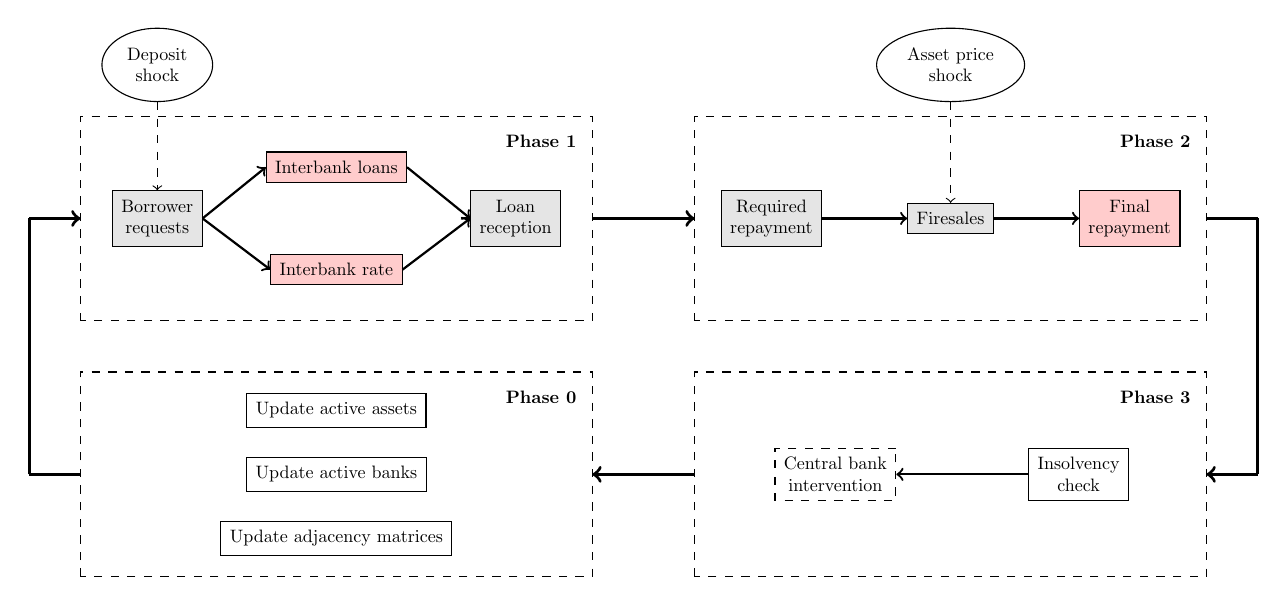
\begin{tikzpicture}[scale=0.65, every node/.style={scale=0.65}]

%%%%%%%%%%%%%%%%%%%%%%%%%%%%%%%%%%%%%%%%%%%%%%%%%%%%%%%%%%%%%%%%
% Phase 0
%%%%%%%%%%%%%%%%%%%%%%%%%%%%%%%%%%%%%%%%%%%%%%%%%%%%%%%%%%%%%%%%

% Border
\draw [dashed] (2,-3) rectangle (12,1);
\node[] (p2) at (11,0.5) {\textbf{Phase 0}};

% Different components

\node[fill=none,draw,align=center,inner sep = 5pt] (p1_AM) at (7,-1) {Update active banks};

\node[fill=none,draw,align=center,inner sep = 5pt] (p1_AM) at (7,0.25) {Update active assets};

\node[fill=none,draw,align=center,inner sep = 5pt] (p0_AB) at (7,-2.25) {Update adjacency matrices};


%%%%%%%%%%%%%%%%%%%%%%%%%%%%%%%%%%%%%%%%%%%%%%%%%%%%%%%%%%%%%%%%
% Phase 1
%%%%%%%%%%%%%%%%%%%%%%%%%%%%%%%%%%%%%%%%%%%%%%%%%%%%%%%%%%%%%%%%

% Border
\draw [dashed] (2,2) rectangle (12,6);
\node[] (p1) at (11,5.5) {\textbf{Phase 1}};

% Different components
\node[fill=gray!20,draw,align=center,inner sep = 5pt] (p1_BR) at (3.5,4) {Borrower \\ requests};

\node[fill=red!20,draw,align=center,inner sep = 5pt] (p1_IBL) at (7,5) {Interbank loans};

\node[fill=red!20,draw,align=center,inner sep = 5pt] (p1_IBR) at (7,3) {Interbank rate};

\node[fill=gray!20,draw,align=center,inner sep = 5pt] (p1_LR) at (10.5,4) {Loan \\reception};

% Shock
\node[align=center,draw,ellipse,inner sep=5pt] (dshock) at (3.5,7) {Deposit \\ shock};
\draw[->,dashed] (dshock.south) -- (p1_BR.north);

% Edges
\draw[->,thick] (p1_BR.east) -- (p1_IBL.west);
\draw[->,thick] (p1_BR.east) -- (p1_IBR.west);
\draw[->,thick] (p1_IBL.east) -- (p1_LR.west);
\draw[->,thick] (p1_IBR.east) -- (p1_LR.west);

%%%%%%%%%%%%%%%%%%%%%%%%%%%%%%%%%%%%%%%%%%%%%%%%%%%%%%%%%%%%%%%%
% Phase 2
%%%%%%%%%%%%%%%%%%%%%%%%%%%%%%%%%%%%%%%%%%%%%%%%%%%%%%%%%%%%%%%%

% Border
\draw [dashed] (14,2) rectangle (24,6);
\node[] (p2) at (23,5.5) {\textbf{Phase 2}};

% Different components
\node[fill=gray!20,draw,align=center,inner sep = 5pt] (p2_RR) at (15.5,4) {Required\\ repayment};

\node[fill=gray!20,draw,align=center,inner sep = 5pt] (p2_FS) at (19,4) {Firesales};

\node[fill=red!20,draw,align=center,inner sep = 5pt] (p2_FR) at (22.5,4) {Final \\repayment};

% Shock
\node[align=center,draw,ellipse,inner sep=5pt] (apshock) at (19,7) {Asset price \\ shock};
\draw[->,dashed] (apshock.south) -- (p2_FS.north);

% Edges
\draw[->,thick] (p2_RR.east) -- (p2_FS.west);
\draw[->,thick] (p2_FS.east) -- (p2_FR.west);

%%%%%%%%%%%%%%%%%%%%%%%%%%%%%%%%%%%%%%%%%%%%%%%%%%%%%%%%%%%%%%%%
% Phase 3
%%%%%%%%%%%%%%%%%%%%%%%%%%%%%%%%%%%%%%%%%%%%%%%%%%%%%%%%%%%%%%%%

% Border
\draw [dashed] (14,-3) rectangle (24,1);
\node[] (p2) at (23,0.5) {\textbf{Phase 3}};

% Different components
\node[fill=none,draw,align=center,inner sep = 5pt] (p3_IS) at (21.5,-1) {Insolvency\\ check};

\node[fill=none,draw,dashed,align=center,inner sep = 5pt] (p3_CBI) at (16.75,-1) {Central bank\\ intervention};

% Edges
\draw[->,thick] (p3_IS.west) -- (p3_CBI.east);

%%%%%%%%%%%%%%%%%%%%%%%%%%%%%%%%%%%%%%%%%%%%%%%%%%%%%%%%%%%%%%%%
% Interphase arrows
%%%%%%%%%%%%%%%%%%%%%%%%%%%%%%%%%%%%%%%%%%%%%%%%%%%%%%%%%%%%%%%%

% 1 --> 2
\draw[->,very thick] (12,4) to (14,4);

% 2 --> 3
\draw[very thick] (24,4) to (25,4);
\draw[very thick] (25,4) to (25,-1);
\draw[->,very thick] (25,-1) to (24,-1);

% 3 --> 0
\draw[->,very thick] (14,-1) to (12,-1);

% 0 --> 1
\draw[very thick] (2,-1) to (1,-1);
\draw[very thick] (1,-1) to (1,4);
\draw[->,very thick] (1,4) to (2,4);

\end{tikzpicture}
\end{document}
